\documentclass[12pt]{article}
\usepackage[utf8]{inputenc}
\usepackage{float}
\usepackage{amsmath}
\usepackage[hmargin=3cm,vmargin=6.0cm]{geometry}
%\topmargin=0cm
\topmargin=-2cm
\addtolength{\textheight}{6.5cm}
\addtolength{\textwidth}{2.0cm}
%\setlength{\leftmargin}{-5cm}
\setlength{\oddsidemargin}{0.0cm}
\setlength{\evensidemargin}{0.0cm}
%misc libraries goes here
\usepackage{tikz}

\begin{document}
\section*{Student Information } 
%Write your full name and id number between the colon and newline
%Put one empty space character after colon and before newline
Full Name : Ahmet Eren Çolak \\
Id Number : 2587921 \\

% Write your answers below the section tags
\section*{Q. 1}
Using Prim’s algorithm:
\subsection*{a.}
\begin{center}
    \setlength{\tabcolsep}{18pt}
    \begin{tabular}{ccc}
        \textbf{Choice}     & \textbf{Edge}     & \textbf{Weight} \\
        1                   & \{e, f\}          & 1      \\
        2                   & \{e, h\}          & 2      \\
        3                   & \{g, h\}          & 2      \\
        4                   & \{d, g\}          & 3      \\
        5                   & \{d, a\}          & 2      \\
        6                   & \{d, b\}          & 3      \\
        7                   & \{f, c\}          & 3      \\
        8                   & \{h, i\}          & 4     
    \end{tabular}
\end{center}
   
\subsection*{b.}
\begin{center}
    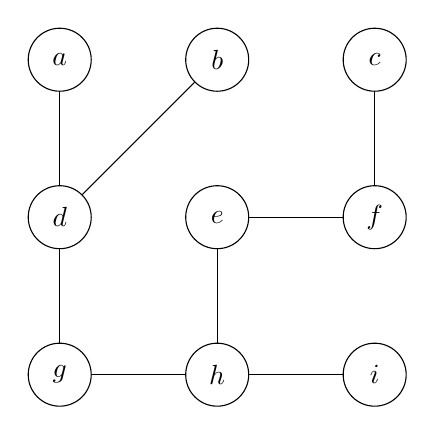
\begin{tikzpicture}
        \node[draw,circle,minimum size=0.8cm,inner sep=0pt] (a) at (0,0) {$a$};
        \node[draw,circle,minimum size=0.8cm,inner sep=0pt] (b) at (2,0) {$b$};
        \node[draw,circle,minimum size=0.8cm,inner sep=0pt] (c) at (4,0) {$c$};
        \node[draw,circle,minimum size=0.8cm,inner sep=0pt] (d) at (0,-2) {$d$};
        \node[draw,circle,minimum size=0.8cm,inner sep=0pt] (e) at (2,-2) {$e$};
        \node[draw,circle,minimum size=0.8cm,inner sep=0pt] (f) at (4,-2) {$f$};
        \node[draw,circle,minimum size=0.8cm,inner sep=0pt] (g) at (0,-4) {$g$};
        \node[draw,circle,minimum size=0.8cm,inner sep=0pt] (h) at (2,-4) {$h$};
        \node[draw,circle,minimum size=0.8cm,inner sep=0pt] (i) at (4,-4) {$i$};
        \draw (a) -- (d) -- (g) -- (h) -- (i);
        \draw (d) -- (b);
        \draw (h) -- (e) -- (f) -- (c);
    \end{tikzpicture}
\end{center}

\subsection*{c.}
In general, the minimum spanning tree is not unique for any connected edge-weighted undirected graph. Because if there are multiple minimum weighted edge and they form a circuit when they exist together, there will be multiple minimum spanning trees for that graph. In this case, graph $G$ is unique because there is no example of this situation.
\subsection*{d.}
According to Prim’s algorithm, the first added edge to the minimum spanning tree is the one with the minimum weight. Hence, if minimum-weight edge of a graph is unique then it has to be in the minimum spanning tree.
\section*{Q. 2}
Yes, $G$ and $H$ are isomorphic because graph $G$ can be drawn with the vertices of the graph $H$:
\begin{center}
    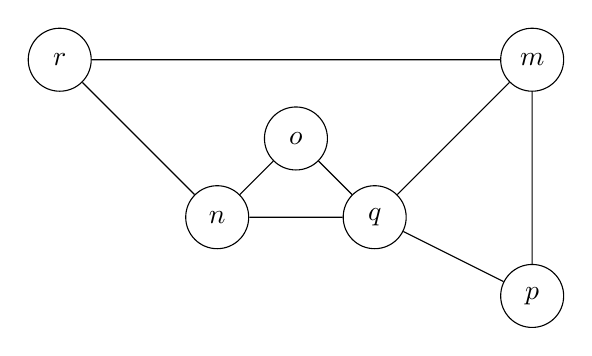
\begin{tikzpicture}
        \node[draw,circle,minimum size=0.8cm,inner sep=0pt] (r) at (0,0) {$r$};
        \node[draw,circle,minimum size=0.8cm,inner sep=0pt] (n) at (2,-2) {$n$};
        \node[draw,circle,minimum size=0.8cm,inner sep=0pt] (o) at (3,-1) {$o$};
        \node[draw,circle,minimum size=0.8cm,inner sep=0pt] (q) at (4,-2) {$q$};
        \node[draw,circle,minimum size=0.8cm,inner sep=0pt] (p) at (6,-3) {$p$};
        \node[draw,circle,minimum size=0.8cm,inner sep=0pt] (m) at (6,0) {$m$};
        \draw[xshift=-1cm] (m) -- (r) -- (n) -- (o) -- (q) -- (p) -- (m) -- (q) -- (n);
    \end{tikzpicture}
\end{center}

\section*{Q. 3}
\subsection*{a.}
Vertices: 7, Edges: 6, Height: 3
\subsection*{b.}
Preorder traversal: p, q, r, s, t,u, v \\
Inorder traversal: q, p, s, r, u, t, v \\
Postorder traversal: q, s, u, v, t, r, p 
\subsection*{c.}
Since each internal vertex has exactly $2$ children, T is a full binary tree.
\subsection*{d.}
No, T is not a complete binary tree because nodes of tree is at right as possible as it can be and second level is not filled.
\subsection*{e.}
T is not a balanced binary tree because there is a leaf at the level 1. 
\subsection*{f.}
T is a binary search tree because each key of vertices is larger than the keys of vertices it its left subtree and smaller than the keys of all vertices in its right subtree.
\subsection*{g.}
To have a full binary tree with minimum vertices and height 5, imagine the tree with minimum vertices and height 5:
\begin{center}
    \begin{tikzpicture}[nodes={draw, circle}]
        \node[circle,fill,inner sep=1pt] at (0,0) (a) { };
        \node[circle,fill,inner sep=1pt, below left of=a](b) { };
        \node[circle,fill,inner sep=1pt, below left of=b](c) { };
        \node[circle,fill,inner sep=1pt, below left of=c](d) { };
        \node[circle,fill,inner sep=1pt, below left of=d](e) { };
        \node[circle,fill,inner sep=1pt, below left of=e](f) { };
        \draw[xshift=-1cm] (a) -- (b) -- (c) -- (d) -- (e) -- (f);
    \end{tikzpicture}
\end{center}
To make it full binary tree, each vertex except the leaf at the bottom must have one more child:
\begin{center}
    \begin{tikzpicture}[nodes={draw, circle}]
        \node[circle,fill,inner sep=1pt] at (0,0) (a) { };
        \node[circle,fill,inner sep=1pt, below left of=a](b) { };
        \node[circle,fill,inner sep=1pt, below left of=b](c) { };
        \node[circle,fill,inner sep=1pt, below left of=c](d) { };
        \node[circle,fill,inner sep=1pt, below left of=d](e) { };
        \node[circle,fill,inner sep=1pt, below left of=e](f) { };
        \node[circle,fill,inner sep=1pt, below right of=a](p) { };
        \node[circle,fill,inner sep=1pt, below right of=b](q) { };
        \node[circle,fill,inner sep=1pt, below right of=c](r) { };
        \node[circle,fill,inner sep=1pt, below right of=d](s) { };
        \node[circle,fill,inner sep=1pt, below right of=e](t) { };
        \draw[xshift=-1cm] (a) -- (b) -- (c) -- (d) -- (e) -- (f);
        \draw[xshift=-1cm] (a) -- (p);
        \draw[xshift=-1cm] (b) -- (q);
        \draw[xshift=-1cm] (c) -- (r);
        \draw[xshift=-1cm] (d) -- (s);
        \draw[xshift=-1cm] (e) -- (t);
    \end{tikzpicture}
\end{center}
Therefore, there are 11 nodes in a full binary tree with minimum nodes and height 5.
\end{document}